\documentclass[tikz,border=2pt]{standalone}
\usepackage{amsmath}
\usepackage{pgfplots}
\pgfplotsset{compat=1.18}
\usetikzlibrary{arrows.meta}
\begin{document}
% Queue drift: L_0 = 40, arrivals 7,5,6,6,7,5,5,6,7,6 (mean 6), constant capacity mu = 7 (drift -1)
% or mu = 5 (drift +1); the paths end at 30 and 50, near the drift lines 40 - k and 40 + k.
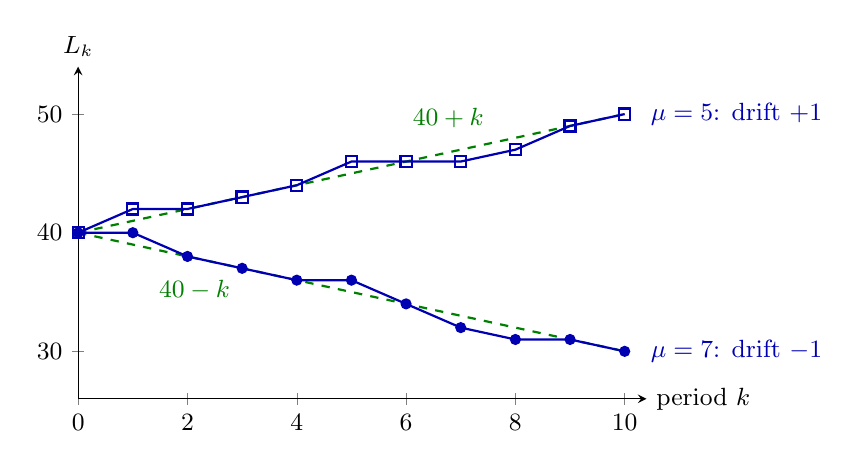
\begin{tikzpicture}[font=\small, >={Latex[length=2mm]}]
  \begin{axis}[
    axis lines=left, xmin=0, xmax=10.4, ymin=26, ymax=54,
    xtick={0,2,4,6,8,10}, ytick={30,40,50},
    xlabel={period $k$}, ylabel={$L_k$},
    xlabel style={at={(axis description cs:1,0)}, anchor=west},
    ylabel style={rotate=-90, at={(axis description cs:0,1)}, anchor=south},
    width=8.8cm, height=5.8cm, clip=false
    ]
    \addplot[green!50!black, thick, dashed, domain=0:10, samples=2] {40-x};
    \addplot[green!50!black, thick, dashed, domain=0:10, samples=2] {40+x};
    \addplot[blue!70!black, thick, mark=*, mark size=1.6pt] coordinates
      {(0,40) (1,40) (2,38) (3,37) (4,36) (5,36) (6,34) (7,32) (8,31) (9,31) (10,30)};
    \addplot[blue!70!black, thick, mark=square, mark size=2pt] coordinates
      {(0,40) (1,42) (2,42) (3,43) (4,44) (5,46) (6,46) (7,46) (8,47) (9,49) (10,50)};
    \node[blue!70!black, anchor=west] at (axis cs:10.3,50) {$\mu=5$: drift $+1$};
    \node[blue!70!black, anchor=west] at (axis cs:10.3,30) {$\mu=7$: drift $-1$};
    \node[green!50!black, anchor=south east] at (axis cs:7.6,48.0) {$40+k$};
    \node[green!50!black, anchor=north west] at (axis cs:1.3,36.8) {$40-k$};
  \end{axis}
\end{tikzpicture}
\end{document}
